\documentclass[11p, titlepage, oneside, a4paper]{article}
% Packages
\usepackage{amsmath}
\usepackage{graphicx}
\usepackage{hyperref}
\usepackage[english,swedish]{babel}
\usepackage[
    backend=biber,
    style=authoryear-ibid,
    sorting=ynt
]{biblatex}
\usepackage[utf8]{inputenc}
\usepackage[T1]{fontenc}
%Källor
\addbibresource{mall.bib}
\graphicspath{ {./images/} }

% Ändra de rader som behöver ändras
\def\inst{Teknikprogrammet}
\def\typeofdoc{Laborationsrapport}
\def\course{Fysik 1 150p}
\def\pretitle{Laboration 1}
\def\title{Rörelse: Hastighet och acceleration}
\def\name{Sam Sperring}
\def\username{samsperring@gmail.com}
\def\email{\username{}}
\def\graders{Magnus Silverdal}

\begin{document}

\begin{titlepage}
		\thispagestyle{empty}
		\begin{large}
			\begin{tabular}{@{}p{\textwidth}@{}}
				\textbf{NTI gymnasiet \hfill \today} \\
				\textbf{\inst} \\
				\textbf{\typeofdoc} \\
			\end{tabular}
		\end{large}
		\vspace{10mm}
		\begin{center}
			\LARGE{\pretitle} \\
			\huge{\textbf{\course}}\\
			\vspace{10mm}
			\LARGE{\title} \\
			\vspace{15mm}
			\begin{large}
				\begin{tabular}{ll}
					\textbf{Namn} & \name \\
					\textbf{E-mail} & \texttt{\email} \\
				\end{tabular}
			\end{large}
			\vfill
            
\includegraphics[width=0.5\textwidth]{images/NTI Gymnasiet_Symbol_print_svart.png}
			\vfill
            \large{\textbf{Handledare}}\\
			\mbox{\large{\graders}}
		\end{center}
	\end{titlepage}

    \begin{otherlanguage}{english}
	\begin{abstract}
        Me and my friend Oscar where given the task to do 2 different experiments involving power. The first experiment was calculating the friction and normal speed of the object with different weights on it. and making a graph out of it to se the connection between all the different weights. we did this by tilting a wooden plank untill the woodblock on top of it with the weights started sliding of at a consistent speed. then we just measured the hight it started sliding on and then we had everything we needed.

        on the second experiment we measured the spring force by adding on different amounts of weights on a spring and seeing how much it extends. We measured this with a ruler in cm and we then looked at the connection between all the differnet weights to make a graph  out of it.

    \end{otherlanguage}
    % Om arbetet är långt har det en innehållsförteckning, annars kan den utelämnas
	\pagenumbering{roman}
	\tableofcontents
	
	% och lägger in en sidbrytning
	\newpage

	\pagenumbering{arabic}
	
	% i Sverige har vi normalt inget indrag vid nytt stycke
	\setlength{\parindent}{0pt}
	% men däremot lite mellanrum
	\setlength{\parskip}{10pt}
	
	\section{Syfte och frågeställning}
	i den första  är syftet at räkna ut friktionen och normal hastiheten på när det gäller olicka vickter och sendan göra en graf på det. i det andra experimentet ska vi räckna ut fjäder kraften på en fjäder vi navänder olicka vickter på fjädern för at göra det senan gör vi en graf på det.

    \section{Metod och materiel upgift 1}
    \begin{enumerate}
        \item planka
        \item träkloss
        \item vickter
        \item mätinstrument
        \item stative
         \end{enumerate}
        vi stälde up plankan på ett stative så den lutade olicka mycket beroende på hur högt stativ pinen är. sen tog vi våran träcloss la den på träplankan och lutade den tills träclossen gled ner i en konstant hastighet vi gjore sama sak med 4 olicka vickter på. vre gång så mätte vi hur högt up plankan va så vi kan gemföra det med all olicka vickter.

        \end{enumerate}
    \section{Metod och materiel upgift 2}
    \begin{enumerate}
        \item stative
        \item fjäder
        \item vickter
        \item något som får vickterna at sita fast i fjäden

        \end{enumerate}
        vi satte up fjädern på starivet så den hänger neråt vi mäte hur lång fjädern va utan vickt och sen la vi på mer och mer vickt och mäte längden på den med dom olicka vickterna.

        \begin{figure}[!h]
            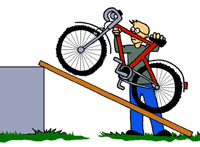
\includegraphics[width=0.8\textwidth]{images/lutandePlan.jpg}
            \caption{En blid hade varit superbra här}
            \label{fig:lutandeplan}
        \end{figure}
        

    \newpage
	\section{Analys och beräkning}
        Datat från analysen av filmen visas i tabell \ref{table:result}
    
        
        \begin{table}
            \begin{center}
            \begin{tabular}{ |c|c| } 
                \hline
                Position (m) & Tid (s)  \\ 
                \hline
                0 & 0  \\ 
                0.1 & 0.02 \\
                \vdots & \vdots \\
                \hline
            \end{tabular}
                \caption{Mätvärden}
                \label{table:result}
            \end{center}
        \end{table}            
        

    Datat importeras i Excel och hastigheten beräknas med hjälp av formeln
    \begin{equation}
        v_m = \frac{\Delta s}{\Delta t}
    \end{equation}
    
    \section{Slutsats och resultat} 
        Resultatet av beräkningarna illustreras i graferna 2 och 3
    \section{Diskussion} 
    Resultatet är perfekt...

    
    \printbibliography

\end{document}

